%---------------------------------------------------------------------
%
%                          Cap�tulo 5
%
%---------------------------------------------------------------------

\chapter{Implementation Study}

\begin{FraseCelebre}
\begin{Frase}
Time of your life
\end{Frase}
\begin{Fuente}
Thomas \& Guy-Manuel, Daft Punk
\end{Fuente}
\end{FraseCelebre}


\begin{resumen}
In this chapter, tasks related to the physical implementation of the platform are described. These tasks cover from the layout design, 3D modelling, and GERBER files generation, to the final components mounting on the . Decisions about components or layout designs, and final results are exposed.  
\end{resumen}



%-------------------------------------------------------------------
\section{Introduction}
%-------------------------------------------------------------------
\label{cap5:sec:introduction}
%------------------------------------------------------------------

Once the system is designed over a logic circuitry level, it is moment to build a \ac{PCB} design responsive to the developed schematics. This process includes the PCB dimmenssions, components placement, tracks routing, silkscreens, etc. These tasks are achieved over the Altium Designer, same software described in Section \ref{cap4:sec:altiumDesigner}.

All the implementations share some common features regarding their layout designs. On the one hand, the used components will keep, whenever possible\footnote{Some components do not offer SMD packaging due to their electric properties.}, \ac{SMD} packaging. This technology gives a more reduced size and supports lower power ratings. Precissely, the \ac{SMD} package used for most of two-terminal components is the 0603 (1608 metric) size\footnote{1.6 mm x 0.8 mm (0.063 in x 0.031 in). Typical power rating for resistors are 0.1 watt.} Figure \ref{fig:cap5:smdsizes} shows a classification for two-terminal \ac{SMD} components in metrics and imperial units.

\begin{figure}
        \centering
                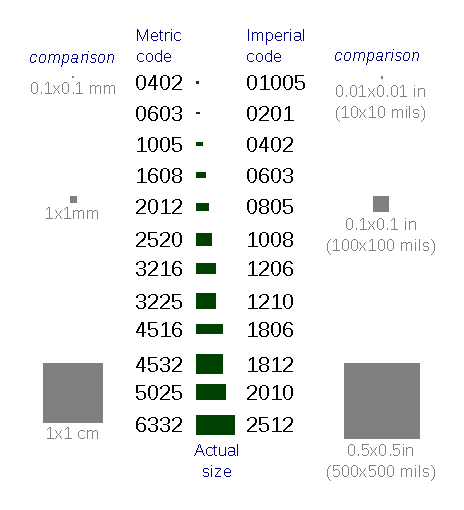
\includegraphics{Imagenes/Vectorial/Capitulo5/smdsizes}
        \caption{Two-terminal SMD packages classification.}
        \label{fig:cap5:smdsizes}
\end{figure}

All the created layouts are built over two-layer boards. Two layers are enough for our purposes since they allow to place the components in a sufficiently reduced area and power planes are not required. More layers, in addition, would increase significantly the board costs. 

For the tracks routing process, some considerations are taken. Ground planes are placed to face noise reduction, this way a low impedance way is provided for the power signals. Moreover, parasitic \ac{EM} emissions are reduced. Power tracks are width enough to support the supplied current flow.

Together with the layout deployment, Altium Designer offers the chance to embbed 3D models of each component, building up eventually a whole 3D model of the complete board. This tool was employed, and 3D models were rendered, obtaining a preview of the modules on advance to their materialization.

\ac{PCB} manufacturer, PCBCART\footnote{www.pcbcart.com} will produce the \ac{PCB}s from the outputed fabrication files. Final \ac{PCB} posses a 1.6 mm thickness, and copper layers are 35 $\mu$m thick. 

%-------------------------------------------------------------------
\subsection{Mounting}
%-------------------------------------------------------------------
Small package components, like the employed here, requires for precission tools to be mounted. Proper tweezers are helpful dealing with components. The soldering station used is a JBC AM 6000 ************REF, offering several soldering tips on the 1-4 mm diameter and useful tools as hot tweezers or desoldering accesories. Binocular loupe ************** WHATEVER ************ is essential for better precission. 

Components use to include at their datasheets guidelines about their surrounding layout, soldering tips, or mounting processes. They are reviewed and taken into account for the proccess.

The secuential mounting, and the existing firmware allow to carry through simple tests to ckeck proper functionality and detect errors. Actually, several corrections and adjustments were made during the mounting task.  

%-------------------------------------------------------------------
\section{Transceivers - $\mu$Trans 434/868}
%-------------------------------------------------------------------
\label{cap5:sec:transceivers}
%------------------------------------------------------------------

\figura{Vectorial/Todo}{width=0.4\textwidth}{fig:cap5:mtrans3dmodel}%
{$\mu$Trans 434/868 3D model.}

%-------------------------------------------------------------------
\subsection{Description}
%-------------------------------------------------------------------

This module was developed because of the non-existance of reduced size \ac{RI}s including the MRF49XA transceiver, so, by definition, the module must posses a reduced size. Taking advantage of the included MRF24j40MA \ac{RI}, it was decided to design a \ac{PCB} module fitting the footprint of the named \ac{RI}. This way a single footprint is commont to all the included \ac{RI}s. This footprint is defined in Figure \ref{fig:cap5:mtransfootprint}.

\begin{figure}
        \centering
                
\includegraphics{Imagenes/Vectorial/Todo}
        \caption{$\mu$Trans 434/868 and MRF24j40MA shared footprint.}
        \label{fig:cap5:mtransfootprint}
\end{figure}

The \ac{PCB} size must be suitable for this footprint, not exceeding its width. $\mu$Trans \ac{PCB} shape is defined as in Figure \ref{fig:cap5:mtransshape}.

\begin{figure}
        \centering
                
\includegraphics{Imagenes/Vectorial/Todo}
        \caption{$\mu$Trans 434/868 \ac{PCB} shape.}
        \label{fig:cap5:mtransshape}
\end{figure}

Module pads are based vias\footnote{A via is a electrical connection between layers in a physical electronic circuit that goes through the plane of one or more adjacent layers.}, with a ******* mm rad. through hole. These holes are width enouth let the solder tip into them and solder the pads over the footprint. These pads constitute the electrical interface between the $\mu$Trans and \ac{CNGD} and suppose a low-cost and size solution.  

MRF49XA datasheet provides hints for the inclussion of the transceiver into a \ac{PCB}. It recommends to fill area underneath the transceiver with ground vias, thereby the module includes such vias. In addition, to have an easily accessible measure of the clock signal, the top layer posses a small pad that provides this signal. Minimal spacing is set to ****************** and the standard track width is *********************** . Power tracks width is set to *********** and ground planes are placed on top and botton layers. Vias through holes minimal radium are ************width. Table \ref{tab:cap5:mtranscomponents} contains the needed components for the $\mu$Trans 434/868 on both versions.

\begin{table}[h]
\centering
\scalebox{0.7}{
\begin{tabular}{||c | c ||}
\hline \\
\hline \\
\hline \\
\hline \\

\end{tabular}
}
\caption{Component description for $\mu$Trans 434/868.%
         \label{tab:cap5:mtranscomponents}}
\end{table} 

%-------------------------------------------------------------------
\subsection{Layout}
%-------------------------------------------------------------------
Different layers of the layout can be obseved at Appendix \ref{ap2:layout}. Figures \ref{} and \ref{} show the top and botton copper layers respectively. Figures \ref{} and \ref{} give the view of the top and botton silkscreens respectively.

%-------------------------------------------------------------------
\subsection{Prototype testing}
%-------------------------------------------------------------------

Basic tests to check proper functionality were made while prototyping the module.

Firstly, the modules were tested over the \ac{FCD} platform. For this, the $\mu$Trans pads were wired and connected to header prepared for the MRF49XA PICtail Plus Daughter Board. On this platform and using an multi-probe oscilloscope ********************************, \ac{SPI} communication signals and other were checked, and possible errors debbuged.

After this, and in collaboration with other MRF49XA modules, it was checked that the module properly carried out handshaking, network detection and joining, and data transmission and reception processes.

%-------------------------------------------------------------------
\subsection{Final Result}
%-------------------------------------------------------------------

\figura{Vectorial/Todo}{width=0.4\textwidth}{fig:cap5:mtransfront}%
{Detailed front view of the $\mu$Trans module.}

\figura{Vectorial/Todo}{width=0.4\textwidth}{fig:cap5:mtransback}%
{Detailed back view of the $\mu$Trans module.}

%-------------------------------------------------------------------
\section{Main Board - cognitiveNextGenerationDevice}
%-------------------------------------------------------------------
\label{cap5:sec:currentDevices}
%-------------------------------------------------------------------

\figura{Vectorial/Todo}{width=0.4\textwidth}{fig:cap5:cngd3dmodel}%
{cNGD 3D model.}

%-------------------------------------------------------------------
\subsection{Description}
%-------------------------------------------------------------------
The \ac{CNGD} \ac{PCB} has to implement the whole design described in Section \ref{cap4:sec:cNGD} attending to expand functionality and usability, and reducing size and cost. Since this is key board of the whole system, most part of the weight ot the operation requirements relies on it. It must mainly contain the three \ac{RI}s, give support to expansion modules, include the power supply and battery room, programming system, and microcontroller. In addition, it must provide an easy access to the control modules (leds and push buttons) and easy deployment. Regading its test-bed character, the module must include some kind of anchors to fix it anywhere or incrust some feet. All these features must be achieved keeping size and cost limited, so the module become affordable and valuable. Figure \ref{fig:cap5:cngdshape} shows the \ac{PCB} shape.

\begin{figure}
        \centering
                
\includegraphics{Imagenes/Vectorial/Todo}
        \caption{cNGD \ac{PCB} shape.}
        \label{fig:cap5:cngdshape}
\end{figure}

Power supply system, $\mu$USB and PGE connector are gathered together as entire interfacing slot at large edge 2 of the \ac{PCB}. \ac{RI}s are thought to be placed at the three short edges. 434 MHz \ac{RI} at edge 1, 868 MHZ \ac{RI} at edge 2 and 2.4 GHz \ac{RI} at edge 3. Figure \ref{fig:cap5:cngdfront} can give a better view of these ideas.  

The board includes four holes for the battery to be attached. Figure \ref{}***** ilustrates the way it works, for legs fix together the board and the batteries-holder. Moreover, the \ac{PCB} includes for more holes for general purpose in case of feet or fixing are required.

% 2 FIGURAs BATERIAS (2d y 3d)

Headers module has been placed relying on long edges 1 and 2, Figure \ref{}****** shows it. Future expansion modules will be attached to this module through exctly equal headers on them, this way it will be possible to stack several expansion modules ones above others. The headers footprint to include in future expansion modules to fit the design is ilustrated in Figure \ref{}*************.

%FIGURAS HEADERSSSSSSSSSSSSSSSSSSSSS

The minimum spacing among tracks is set to *********, and tracks widths vary on.....*************. Vias through holes are *********. Table \ref{tab:cap5:cngdcomponents} details the needed components for \ac{CNGD} module.

\begin{table}[h]
\centering
\scalebox{0.7}{
\begin{tabular}{||c | c ||}
\hline \\
\hline \\
\hline \\
\hline \\

\end{tabular}
}
\caption{Component description for cNGD.%
         \label{tab:cap5:cngdcomponents}}
\end{table} 
%-------------------------------------------------------------------
\subsection{Layout}
%-------------------------------------------------------------------
Different layers of the layout can be obseved at Appendix \ref{ap2:layout}. Figures \ref{} and \ref{} show the top and botton copper layers respectively. Figures \ref{} and \ref{} give the view of the top and botton silkscreens respectively.
%-------------------------------------------------------------------
\subsection{Prototype testing}
%-------------------------------------------------------------------
When prototyping, first part to test is the right operation of the \ac{MCU}. After solderin R4, C2, the reset circuit, PGE module, and the \ac{MCU} itself, the microcontroller is brought under its first programming. For a right operation, is needed a right software configuration of the \ac{MCU} parameters, choosing the internal clock. 

Once the right programation of the \ac{MCU} is tested, the external clocks are mounted and tested by changing the software parameters. After this check, it is time for push buttons and leds, which are tested using test software described in Section \ref{cap6:sec:testBenches}. Rest of decoupling capacitors around the \ac{MCU} can be soldered.

For these already described checkings, power supply from the ICD3 is used. Next step is to mount the power supply system and, using external sources, try the right operation of the mounted modules.
 
At this point, the need of debbuging traces arises to keep on mounting the device. A serial communication interface is required, and since the used firmware already supports for RS-232 communication, the rs232SHIELD is mounted and used. To read more details about this mounting, go to Section \ref{cap5:sec:rs232shield}. Headers must be soldered on the board to use this shield.

Last, but not least, modules to try are the \ac{RI}s. One by one, they are added to the \ac{CNGD} and checked. The chosen firmware contains several radio tests for general \ac{TX}/\ac{RX}, handshaking, channel switching. The \ac{RI}s can be tested in conjunction with the equivalent \ac{RI}s at the \ac{FCD}.

%-------------------------------------------------------------------
\subsection{Final result}
%-------------------------------------------------------------------
\figura{Vectorial/Todo}{width=0.4\textwidth}{fig:cap5:cngdfront}%
{Detailed front view of the cNGD.}

\figura{Vectorial/Todo}{width=0.4\textwidth}{fig:cap5:cngdback}%
{Detailed back view of the cNGD.}

%-------------------------------------------------------------------
\section{Serial Communication Board - rs232SHIELD}
%-------------------------------------------------------------------
\label{cap5:sec:rs232shield}
%-------------------------------------------------------------------

\figura{Vectorial/Todo}{width=0.4\textwidth}{fig:cap5:rs2323dmodel}%
{rs232SHIELD 3D model.}

%-------------------------------------------------------------------
\subsection{Description}
%-------------------------------------------------------------------

%-------------------------------------------------------------------
\subsection{Layout}
%-------------------------------------------------------------------
Different layers of the layout can be obseved at Appendix \ref{ap2:layout}. Figures \ref{} and \ref{} show the top and botton copper layers respectively. Figures \ref{} and \ref{} give the view of the top and botton silkscreens respectively.
%-------------------------------------------------------------------
\subsection{Prototype testing}
%-------------------------------------------------------------------

%-------------------------------------------------------------------
\subsection{Final results}
%-------------------------------------------------------------------

\figura{Vectorial/Todo}{width=0.4\textwidth}{fig:cap5:rs232front}%
{Detailed front view of the rs232SHIELD module.}

\figura{Vectorial/Todo}{width=0.4\textwidth}{fig:cap5:rs232back}%
{Detailed back view of the rs232SHIELD module.}

%-------------------------------------------------------------------
\section{Battery charger - chargerSHIELD}
%-------------------------------------------------------------------
\label{cap5:sec:chargerShield}
%-------------------------------------------------------------------

\figura{Vectorial/Todo}{width=0.4\textwidth}{fig:cap5:charger3dmodel}%
{chargerSHIELD 3D model.}

%-------------------------------------------------------------------
\subsection{Description}
%-------------------------------------------------------------------

%-------------------------------------------------------------------
\subsection{Layout}
%-------------------------------------------------------------------
Different layers of the layout can be obseved at Appendix \ref{ap2:layout}. Figures \ref{} and \ref{} show the top and botton copper layers respectively. Figures \ref{} and \ref{} give the view of the top and botton silkscreens respectively.
%-------------------------------------------------------------------
\subsection{Prototype testing}
%-------------------------------------------------------------------

%-------------------------------------------------------------------
\subsection{Final results}
%-------------------------------------------------------------------
\figura{Vectorial/Todo}{width=0.4\textwidth}{fig:cap5:chargerfront}%
{Detailed front view of the chargerSHIELD module.}

\figura{Vectorial/Todo}{width=0.4\textwidth}{fig:cap5:chargerback}%
{Detailed back view of the chargerSHIELD module.}


%-------------------------------------------------------------------
\section{Conclusions}
%-------------------------------------------------------------------
\label{cap5:sec:conclusions}
%-------------------------------------------------------------------


%------------------------------------------------------------------
%\section*{\NotasBibliograficas}
%-------------------------------------------------------------------
%\TocNotasBibliograficas

%Citamos algo para que aparezca en la bibliograf�a\ldots
%\citep{ldesc2e}

%\medskip

%Y tambi�n ponemos el acr�nimo \ac{CVS} para que no cruja.

%Ten en cuenta que si no quieres acr�nimos (o no quieres que te falle la compilaci�n en ``release'' mientras no tengas ninguno) basta con que no definas la constante \verb+\acronimosEnRelease+ (en \texttt{config.tex}).


%-------------------------------------------------------------------
%\section*{\ProximoCapitulo}
%-------------------------------------------------------------------
%\TocProximoCapitulo

%...

% Variable local para emacs, para  que encuentre el fichero maestro de
% compilaci�n y funcionen mejor algunas teclas r�pidas de AucTeX
%%%
%%% Local Variables:
%%% mode: latex
%%% TeX-master: "../Tesis.tex"
%%% End:
